\subsection{Userspace: Mesa 3D}

\begin{frame}[t]{Standardized 3D rendering APIs: OpenGL}
  \begin{center}
  \includegraphics[height=4em]{slides/graphics-software-userspace-mesa/opengl-logo.pdf}
  \end{center}

  \begin{itemize}
  \item 3D rendering API, designed for GPU \textbf{hardware acceleration}
    \begin{itemize}
    \item Generic API but \textbf{hardware-specific implementations}
    \item Started by \textbf{Silicon Graphics} in 1992, now managed by the \textbf{Khronos Group}
    \end{itemize}
  \item OpenGL provides a \textbf{high-level approach} to 3D graphics
    \begin{itemize}
    \item Compromise between complexity and fine-grained control
    \item Efficient abstraction, adapted to the hardware
    \item Leaves most memory management to the implementation
    \end{itemize}
  \item \textbf{Stateful} and \textbf{context-based} programming model
  \end{itemize}
\end{frame}

\begin{frame}[t]{Standardized 3D rendering APIs: OpenGL}
  \begin{center}
  \includegraphics[height=4em]{slides/graphics-software-userspace-mesa/opengl-logo.pdf}
  \end{center}

  \begin{itemize}
  \item OpenGL versions evolved with hardware features
    \begin{itemize}
    \item Version 1 targeted fixed-function pipeline GPUs
    \item Version 2 and up allow programming \textbf{vertex and fragment shaders}
    \item More shaders supported with new versions (\textit{geometry, tesselation})
    \end{itemize}
  \item OpenGL comes with the \textbf{GL Shading Language} (GLSL)
    \begin{itemize}
    \item Source code language for OpenGL shaders
    \item C-like syntax with intrinsic functions (e.g. texture access)
    \item Compiled on-the-fly by the GL implementation
    \end{itemize}
  \item Supports \textbf{extensions} that can be queried, for extra features
  \end{itemize}
\end{frame}

\begin{frame}[t]{Standardized 3D rendering APIs: OpenGL ES and EGL}
  \begin{minipage}[t]{0.49\textwidth}
    \centering
    
\includegraphics[height=4em]{slides/graphics-software-userspace-mesa/opengl-es-logo.pdf}
  \end{minipage}
  \hfill
  \begin{minipage}[t]{0.49\textwidth}
    \centering
    
\includegraphics[height=4em]{slides/graphics-software-userspace-mesa/egl-logo.pdf}
  \end{minipage}
  \vspace{0.5em}
  \begin{itemize}
  \item \textbf{OpenGL ES} was introduced as a simplified version for embedded devices
  \item OpenGL ES versions are loosely following OpenGL versions:
    \begin{itemize}
    \item Version 1 targets \textbf{fixed-function} GPUs
    \item Version 2 and up target \textbf{programmable} GPUs
    \end{itemize}
  \item Uses GLSL shaders and the same programming model as OpenGL
  \item \textbf{EGL} was introduced as standardized window integration API
    \begin{itemize}
    \item Connects with the native system display server
    \item Replaces GLX for X11 and adopted as default by Wayland
    \end{itemize}
  \item Supports \textbf{extensions} that can be queried, for extra platform-specific features
  \end{itemize}
\end{frame}

\begin{frame}[t]{Standardized 3D rendering APIs: Vulkan}
  \begin{center}
  \includegraphics[height=4em]{slides/graphics-software-userspace-mesa/vulkan-logo.pdf}
  \end{center}

  \begin{itemize}
  \item \textbf{Vulkan} is a \textbf{low-level} generic API for GPU access
    \begin{itemize}
    \item Started by the Khronos group in 2016 and widely adopted
    \end{itemize}
  \item Suitable for both \textbf{3D rendering} and \textbf{compute}
  \item Uses \textbf{Standard Portable Intermediate Representation} (SPIR-V) shaders
    \begin{itemize}
    \item Unified intermediate representation from (adapted) GLSL/HLSL sources
    \item Compiled with the program instead of on-the-fly (less overhead)
    \item Translated to native GPU operations by implementations
    \end{itemize}
  \item \textbf{Direct programming} model, with low-level \textbf{memory management}
  \item The API provides \textbf{window system integration} (WSI) for many platforms\\
    \textit{e.g. for Wayland: \code{vkCreateWaylandSurfaceKHR}}
  \end{itemize}
\end{frame}

\begin{frame}{Mesa 3D overview}
  \begin{itemize}
  \item Mesa is the reference free software \textbf{3D graphics implementation}
    \begin{itemize}
    \item Started back in 1993, evolved with GPU implementations
    \item Project works with the Khronos Group and develops extensions
    \end{itemize}
  \item Implements support for \textbf{rendering} APIs:
    \begin{itemize}
    \item \textbf{OpenGL} (up to 4.6) and \textbf{OpenGL ES} (up to 3.2)
    \item \textbf{Vulkan} (up to 1.1) with translation to OpenGL via \textbf{Zink}
    \item \textbf{Direct 3D} (version 9 only)
    \end{itemize}
  \item Implements \textbf{windowing system} integration:
    \begin{itemize}
    \item \textbf{EGL} for Wayland, X11, Android, native DRM (GBM) and surface-less
    \item \textbf{Vulkan WSI} for Wayland and X11 (XCB/Xlib)
    \item \textbf{GLX} for X11
    \end{itemize}
  \item Also supports other \textbf{GPU-related features}:
    \begin{itemize}
    \item \textbf{Video decoding} acceleration via VDPAU, VAAPI, OMX
    \item \textbf{Compute} (GPGPU) support via OpenCL (\code{clover})
    \end{itemize}
  \end{itemize}
\end{frame}

\begin{frame}{Mesa 3D implementation highlights}
  \begin{itemize}
  \item Unlike other devices, 3D hardware is \textbf{abstracted in userspace}
    \begin{itemize}
    \item 3D rendering is a very bad fit for in-kernel abstraction
    \item Kernel drivers are much less complicated than GL implementations
    \end{itemize}
  \item Mesa implements driver-specific \textbf{DRM render} support\\
    \begin{itemize}
    \item Manages memory with the GEM and Prime DRM APIs
    \item Manages DRI2 to allow direct rendering
    \end{itemize}
  \item \textbf{Virtual} drivers are also supported (for virtual machines):
    \begin{itemize}
    \item \textbf{vmwgfx}: VMware bridge (proprietary virtual hardware implementation)
    \item \textbf{virgl}: Virtio bridge (standard for Linux and QEMU)
    \end{itemize}
  \item Also provides \textbf{software backends}:
    \begin{itemize}
    \item \textbf{softpipe}: Generic reference software renderer
    \item \textbf{swr}: OpenSWR renderer (for x86 by Intel)
    \item \textbf{llvmpipe}: LLVM-based renderer (high-performance)
    \end{itemize}
  \end{itemize}
\end{frame}

\begin{frame}{Mesa 3D internals: Gallium 3D}
  \begin{itemize}
  \item Classic mesa drivers have significant \textbf{code duplication}:
    \begin{itemize}
    \item API state tracking
    \item Compiler implementation
    \end{itemize}
  \item The Gallium 3D interface splits things up instead:
    \begin{itemize}
    \item \textbf{API State trackers}: maintain the current state for the API in use
    \item \textbf{Drivers}: implement shader compilation and hardware configuration
    \item \textbf{Winsys}: implement low-level kernel interfaces
    \end{itemize}
  \item Gallium drivers implement a pipe interface:
    \begin{itemize}
    \item \code{struct pipe_screen}: textures, buffers and sync management
    \item \code{struct pipe_state}: pipeline configuration and resources state
    \item \code{struct pipe_context}: rendering operation functions
    \end{itemize}
  \item Pipe loaders (DRM or software) select the right pipe driver
  \end{itemize}
\end{frame}

\begin{frame}{Mesa 3D internals: Gallium 3D (illustrated)}
  \begin{center}
  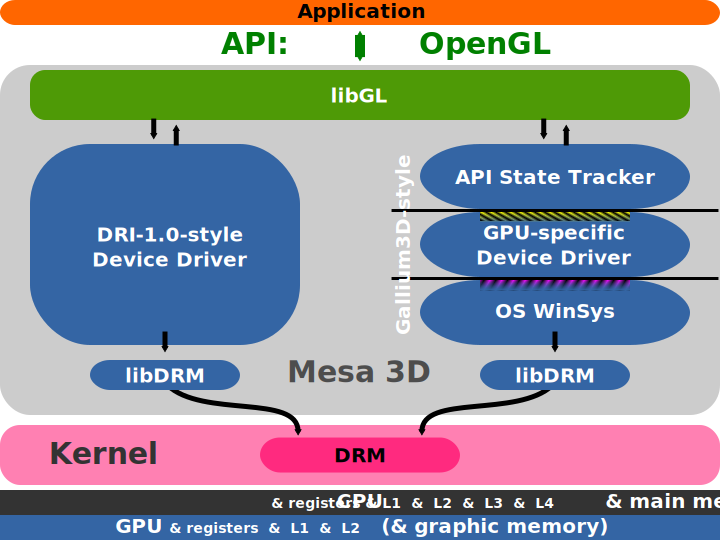
\includegraphics[width=0.5\textwidth]{slides/graphics-software-userspace-mesa/mesa-dri-gallium.pdf}\\
  \textit{\small Driver integration in Mesa 3D}
  \end{center}
\end{frame}

\begin{frame}{Mesa 3D internals: intermediate representations}
  \begin{itemize}
  \item Mesa is in charge of \textbf{compiling shaders} to the native shading ISA
  \item \textbf{Intermediate representations} (IRs) are used for translation
  \item \textbf{Input-level} IRs:
    \begin{itemize}
    \item \textbf{GLSL IR}: Internal GLSL shader representation
    \item \textbf{SPIR-V}: Khronos' Standard Portable Intermediate Representation
    \end{itemize}
  \item \textbf{Internal} IRs:
    \begin{itemize}
    \item \textbf{TGSI IR}: Tungsten Graphics Shader Interface representation
    \item \textbf{NIR}: New efficient internal representation for Mesa
    \item \textbf{Mesa}: Historical implementation (deprecated)
    \end{itemize}
  \item \textbf{External} IR:
    \begin{itemize}
    \item \textbf{LLVM IR}: Used for LLVM interaction (e.g. with llvmpipe)
    \end{itemize}
  \item Drivers emit \textbf{native instructions} from an internal IR and lowering
  \item Once ready, compiled shaders are \textbf{submitted to the GPU}
  \end{itemize}
\end{frame}

\begin{frame}{Mesa 3D internals: intermediate representations (illustrated)}
  \begin{center}
  \includegraphics[width=0.4\textwidth]{slides/graphics-software-userspace-mesa/mesa-ir.pdf}\\
  \textit{\small The Mesa 3D internal representation pipeline}
  \end{center}
\end{frame}

\begin{frame}[fragile]{Mesa 3D Generic Buffer Management}
  \begin{itemize}
  \item Mesa provides a Generic Buffer Management (GBM) interface:
    \begin{itemize}
    \item Buffer creation/destruction (supporting modifiers)
    \item Buffer information (bpp, dimensions, planes, stride, modifiers)
    \item Buffer mapping/unmapping
    \item Buffer dma-buf import/unimport
    \end{itemize}
  \item Compatible with the EGL API:
    \begin{itemize}
    \item \code{struct gbm_device} as \code{EGLNativeDisplayType}
    \item \code{struct gbm_surface} as \code{EGLNativeWindowType}
    \item \code{struct gbm_bo} as \code{EGLNativePixmapType}
    \end{itemize}
  \item Provided with DRM KMS fd for DRI2 (used internally for most operations)\\
  \begin{minted}[fontsize=\small]{console}
struct gbm_device *device = gbm_create_device(drm_fd);
  \end{minted}
  \item Useful when using bare-metal DRM KMS
  \end{itemize}
\end{frame}

\begin{frame}{Mesa 3D hardware support status: desktop}
  \begin{itemize}
  \item Updated Mesa per-driver support at \url{https://mesamatrix.net}
  \item \textbf{Intel HD/Iris Graphics}
    \begin{itemize}
    \item Platforms: Intel only
    \item Mesa driver: i965 (classic), iris (Gallium)
    \item DRM driver: i915
    \item Status: state-of-the art (i965/iris)
    \end{itemize}
  \item \textbf{Nvidia pre-NV110}
    \begin{itemize}
    \item Platforms: Tegra, any PCI-e compatible
    \item Mesa driver: nouveau (Gallium)
    \item DRM driver: nouveau
    \item Status: reverse engineered, advanced
    \end{itemize}
  \end{itemize}
\end{frame}

\begin{frame}{Mesa 3D hardware support status: desktop}
  \begin{itemize}
  \item \textbf{AMD Radeon GCN-ish}
    \begin{itemize}
    \item Platforms: AMD, any PCI-e compatible
    \item Mesa driver: radeonsi (Gallium)
    \item DRM driver: amdgpu
    \item Status: state-of-the art
    \end{itemize}
  \item \textbf{AMD Radeon R600+}
    \begin{itemize}
    \item Platform: AMD, any PCI-e compatible
    \item Driver: r600 (Gallium)
    \item DRM driver: radeon
    \item Status: advanced
    \end{itemize}
  \end{itemize}
\end{frame}

\begin{frame}{Mesa 3D hardware support status: embedded}
  \begin{itemize}
  \item \textbf{Qualcomm Adreno}
    \begin{itemize}
    \item Platforms: Qualcomm Snapdragon
    \item Mesa driver: freedreno (Gallium)
    \item DRM driver: freedreno
    \item Status: reverse engineered, advanced
    \end{itemize}
  \item \textbf{Vivante GCx000}
    \begin{itemize}
    \item Platforms: i.MX6, i.MX8, i.MX8M
    \item Driver: etnaviv (Gallium)
    \item DRM driver: etnaviv
    \item Status: vastly usable
    \end{itemize}
  \end{itemize}
\end{frame}

\begin{frame}{Mesa 3D hardware support status: embedded}
  \begin{itemize}
  \item \textbf{ARM Mali Utgard}
    \begin{itemize}
    \item Platforms: Exynos, Allwinner, Amlogic
    \item Mesa driver: lima (Gallium)
    \item DRM driver: lima
    \item Status: reverse engineered, usable
    \end{itemize}
  \item \textbf{ARM Mali Midgard/Bifrost}
    \begin{itemize}
    \item Platforms: Rockchip, Exynos, Mediatek, Allwinner
    \item Mesa driver: panfrost (Gallium) / PanVK (Vulkan)
    \item DRM driver: panfrost
    \item Status: advanced
    \end{itemize}
  \item \textbf{Imagination PowerVR Rogue}
    \begin{itemize}
    \item Platforms: Mediatek
    \item Mesa driver: imagination
    \item DRM driver: imagination
    \item Status: work in progress
    \end{itemize}
  \end{itemize}
\end{frame}

\begin{frame}{Mesa 3D versus proprietary implementations}
  \begin{itemize}
  \item 3D support is one of the most challenging parts of hardware integration
  \item Proprietary implementations easily lead to various practical issues:
    \begin{itemize}
    \item Lack of support outside of prescribed environments
    \item Lack of specific features or APIs
    \item Lack of maintenance and updates
    \item No adaptation possibility
    \end{itemize}
  \item Mesa provides a collectively-maintained base
    \begin{itemize}
    \item Constantly updated and improved by the community
    \item Easier to manage: works out of the box with distributions
    \end{itemize}
  \item Mesa support is complex and often takes some time to bring performance\\
    \textit{especially for drivers based on reverse-engineering}
  \end{itemize}
\end{frame}

\begin{frame}{Mesa 3D code structure and walkthrough}
  \begin{itemize}
  \item Mesa source code available at: \url{https://gitlab.freedesktop.org/mesa/mesa}
  \item \textbf{Gallium 3D} components:
    \begin{itemize}
    \item Drivers under: \code{src/gallium/drivers/}
    \item Winsys under: \code{src/gallium/winsys/}
    \item API state trackers under: \code{src/gallium/state_trackers/}
    \item Pipe loaders under: \code{src/gallium/auxiliary/pipe-loader/}
    \end{itemize}
  \item \textbf{Compilation and IR} components:
    \begin{itemize}
    \item IR compiler support under: \code{src/compiler/{glsl,nir,spirv}}
    \item TGSI support under: \code{src/gallium/auxiliary/tgsi/}
    \item State tracking between IRs under: \code{src/mesa/state_tracker}
    \end{itemize}
  \item \textbf{Windowing and DRI2} components:
    \begin{itemize}
    \item EGL support under: \code{src/egl/drivers/dri2/}
    \item Vulkan WSI support under: \code{src/vulkan/wsi/}
    \end{itemize}
  \item \textbf{Classic drivers} (DRI-1-style) under: \code{src/mesa/drivers/dri/}
  \item \textbf{GBM} support under: \code{src/gbm/}
  \end{itemize}
\end{frame}

\begin{frame}[fragile]{Mesa 3D hardware support: debug and documentation}
  \begin{itemize}
  \item Mesa is debugged with numerous \textbf{environment variables}
    \begin{itemize}
    \item Generic and per-driver, see \url{https://www.mesa3d.org/envvars.html}
    \item Shader-related, see \url{https://www.mesa3d.org/shading.html}
    \item \code{LIBGL_DEBUG=verbose} for OpenGL, \code{EGL_LOG_LEVEL=debug} for EGL
    \end{itemize}
  \item \code{eglinfo} and \code{glxinfo} show information about the implementation
  \item \textbf{Community} contact:
    \begin{itemize}
    \item Mailing list: \code{dri-devel@lists.freedesktop.org}
    \item IRC channel: \code{#dri-devel} on the OFTC network
    \end{itemize}
  \item \textbf{Documentation} resources:
    \begin{itemize}
    \item Online website: \url{https://www.mesa3d.org/}
    \item Gallium 3D wiki: \url{https://www.freedesktop.org/wiki/Software/gallium/}
    \item Gallium 3D documentation: \url{https://gallium.readthedocs.io/}
    \item Source code reference: \url{https://elixir.bootlin.com/mesa/latest/source}
    \end{itemize}
  \end{itemize}
\end{frame}

\begin{frame}{Graphics software online references}
  \small
  \begin{minipage}[t]{0.45\textwidth}
  \begin{itemize}
  \item Linux man pages
  \item Wikipedia (\url{https://en.wikipedia.org/}):
    \begin{itemize}
    \item \href{https://en.wikipedia.org/wiki/X_Window_System}{X Window System}
    \item \href{https://en.wikipedia.org/wiki/X.Org_Server}{X.Org Server}
    \item \href{https://en.wikipedia.org/wiki/Wayland_(display_server_protocol)}{Wayland (display server protocol)}
    \item \href{https://en.wikipedia.org/wiki/Mesa_(computer_graphics)}{Mesa (computer graphics)}
    \item \href{https://en.wikipedia.org/wiki/OpenGL}{OpenGL}
    \item \href{https://en.wikipedia.org/wiki/Vulkan_(API)}{Vulkan (API)}
    \end{itemize}
  \end{itemize}
  \end{minipage}
  \hfill
  \begin{minipage}[t]{0.5\textwidth}
  \begin{itemize}
  \item Freedesktop.org (\url{https://freedesktop.org/}):
    \begin{itemize}
    \item \href{https://dri.freedesktop.org/wiki/}{Direct Rendering Infrastructure}
    \item \href{https://dri.freedesktop.org/wiki/DRM/}{DRM}
    \item \href{https://wayland.freedesktop.org/}{Wayland}
    \item \href{https://www.x.org/wiki/}{X.org wiki}
    \end{itemize}
  \item Khronos (\url{https://khronos.org/}):
    \begin{itemize}
    \item \href{https://www.khronos.org/opengl/}{OpenGL}
    \item \href{https://www.khronos.org/opengl/wiki/}{OpenGL Wiki}
    \item \href{https://www.khronos.org/egl/}{EGL}
    \item \href{https://www.khronos.org/vulkan/}{Vulkan}
    \end{itemize}
  \end{itemize}
  \end{minipage}
\end{frame}

\begin{frame}{Graphics software illustrations attributions}
  \small
  \begin{itemize}
  \item \href{https://commons.wikimedia.org/wiki/File:X11.svg}{X11 logo: public domain}
  \item \href{https://commons.wikimedia.org/wiki/File:Wayland_Logo.svg}{Wayland logo: Kristian Høgsberg}
  \item \href{https://commons.wikimedia.org/wiki/File:GTK_logo.svg}{GTK logo: Andreas Nilsson, CC BY-SA 3.0}
  \item \href{https://commons.wikimedia.org/wiki/File:GTK_logo.svg}{Qt logo: Qt Project, public domain}
  \item \href{https://commons.wikimedia.org/wiki/File:SDL_Logo.svg}{SDL logo: Arne Claus / SDL Project, public domain}
  \item \href{https://commons.wikimedia.org/wiki/File:Gnomelogo.svg}{GNOME logo: GNOME Foundation, GNU LGPL 2.1+}
  \item \href{https://commons.wikimedia.org/wiki/File:KDE_logo.svg}{KDE logo: KDE e.V., GNU LGPL 2.1+}
  \item \href{https://commons.wikimedia.org/wiki/File:Xfce_logo.svg}{XFCE logo: Xfce Team, GNU LGPL 2.1+}
  \item \href{https://commons.wikimedia.org/wiki/File:Enlightenment_logo_black.png}{Enlightenment logo: Carsten Haitzler and various contributors, BSD}
  \end{itemize}
\end{frame}

\begin{frame}{Graphics software illustrations attributions}
  \small
  \begin{itemize}
  \item \href{https://commons.wikimedia.org/wiki/File:Devuan_GNU-Linux_-_tty_login_-_server_rack.jpg}{Devuan GNU-Linux - tty login - server rack: Francesco Magno, CC BY-SA 4.0}
  \item \href{https://commons.wikimedia.org/wiki/File:DRM_architecture.svg}{DRM architecture: Javier Cantero CC BY-SA 4.0}
  \item \href{https://wayland.freedesktop.org/architecture.html}{Wayland architecture: Wayland Developers, GNU GPL 2+}
  \item \href{https://wayland.freedesktop.org/architecture.html}{X architecture: Wayland Developers, GNU GPL 2+}
  \item \href{https://commons.wikimedia.org/wiki/File:Wayland_display_server_protocol.svg}{Wayland display server protocol: Shmuel Csaba Otto Traian, CC BY-SA 3.0}
  \item \href{https://commons.wikimedia.org/wiki/File:The_Linux_Graphics_Stack_and_glamor.svg}{The Linux Graphics Stack and glamor: Shmuel Csaba Otto Traian, CC BY-SA 3.0}
  \item \href{https://www.khronos.org/assets/utilities/retrieveFile.php?d=opengl&t=logopacks}{Khronos logo pack}
  \item \href{https://commons.wikimedia.org/wiki/File:Gallium3D_vs_DRI_graphics_driver_model.svg}{Gallium3D vs DRI graphics driver model, CC BY-SA 3.0}
  \end{itemize}
\end{frame}
